\chapter{Additional tables and plot from Chapter~\ref{reflectometry2}}

\ref{refl2app}

This appendix contains additional plots and tables associated with Chapter~\ref{reflectometry2}. 
Figures~\ref{fig:dspcccref20}-\ref{fig:dspcccref50} give the NR and SLD profiles for the chemically-consistent model alongside those obtained directly from MD simulations at an APM associated with surface pressures of \SIlist{20;40;50}{\milli\newton\per\meter}.
The equivalent data at a APM associated with a surface pressure of \SI{30}{\milli\newton\per\meter} can be found in Figure~\ref{tab:dspcccref30}. 
%
\begin{figure}
    \centering
    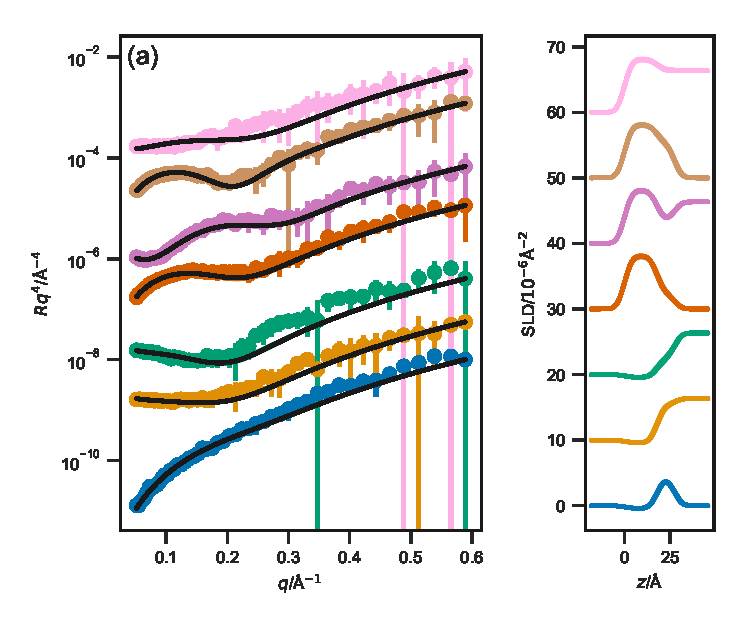
\includegraphics[width=0.49\textwidth]{reflectometry2/dspc_20_ref_sld}
    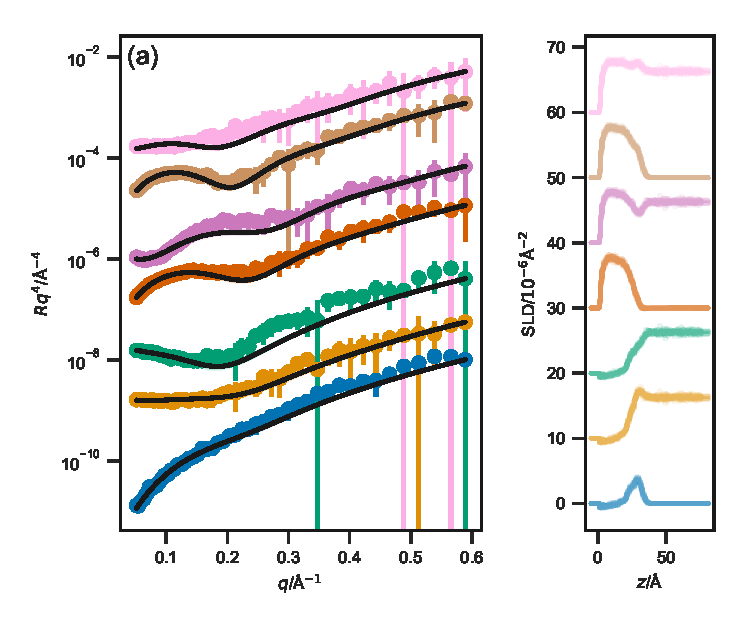
\includegraphics[width=0.49\textwidth]{reflectometry2/dspc_slipids_20_ref_sld}\\
    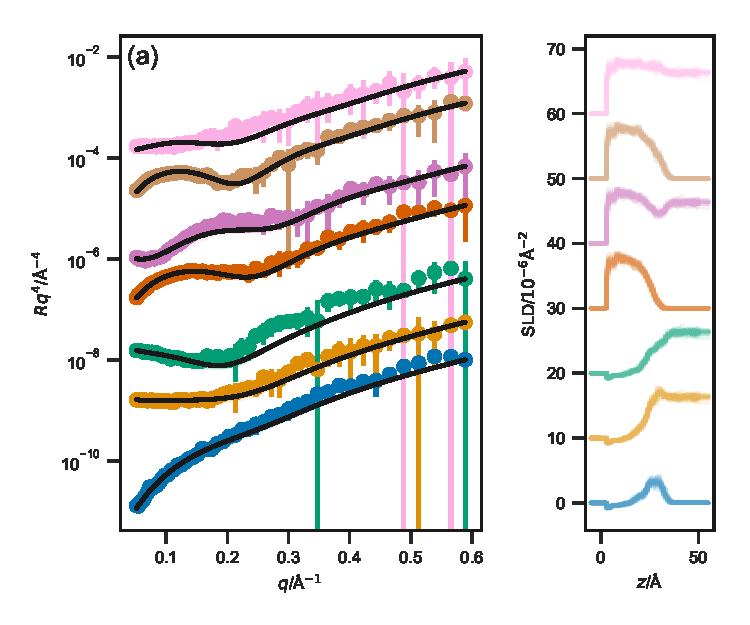
\includegraphics[width=0.49\textwidth]{reflectometry2/dspc_berger_20_ref_sld}
    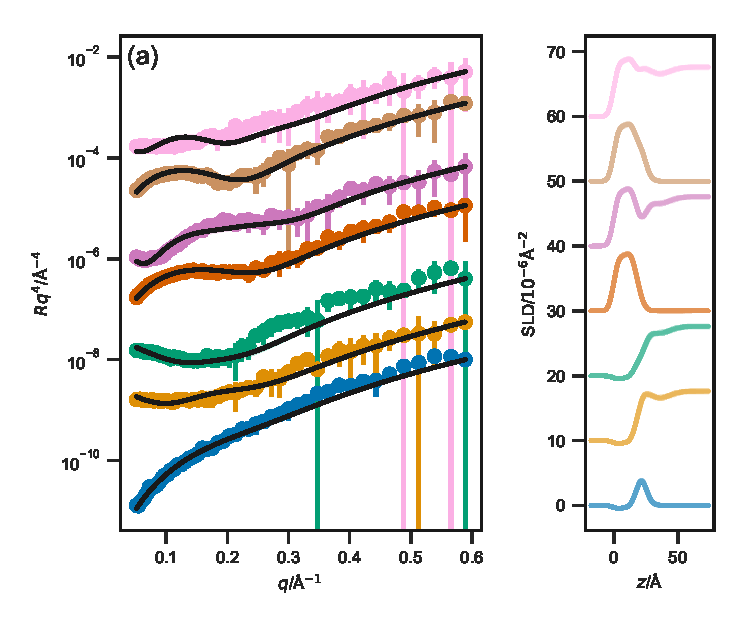
\includegraphics[width=0.49\textwidth]{reflectometry2/dspc_martini_20_ref_sld}
    \caption{The NR profiles (left) and SLD profiles (right) determined at an APM assocaited with a surface pressure of \SI{20}{\milli\newton\per\meter} for; (a) the chemically-consistent model, (b) the Slipid all-atom potential model simulations, (c) the Berger united-atom potential model simulations, and (d) the MARTINI coarse-grained potential model simulations. From top-to-bottom the contrasts are as follows; d$_{83}$-\ce{D2O}, d$_{83}$-ACMW, d$_{70}$-\ce{D2O}, d$_{70}$-ACMW, h-\ce{D2O}, d$_{13}$-\ce{D2O}, d$_{13}$-ACMW. The different contrast NR profiles have been offset in the \emph{y}-axis by an order of magnitude and the SLD profiles offset in the \emph{y}-axis by \SI{10e-6}{\per\angstrom\squared}, for clarity.}
    \label{fig:dspcccref20}
\end{figure}
%
%
\begin{figure}
    \centering
    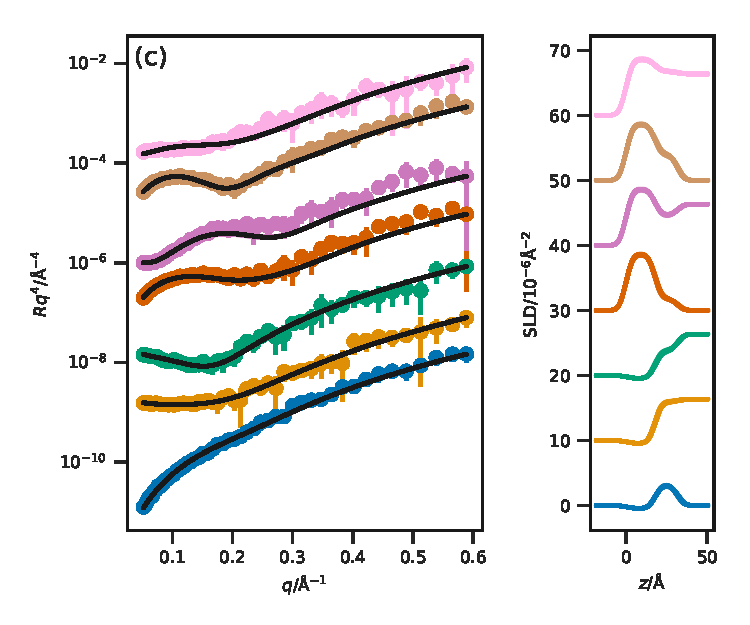
\includegraphics[width=0.49\textwidth]{reflectometry2/dspc_40_ref_sld}
    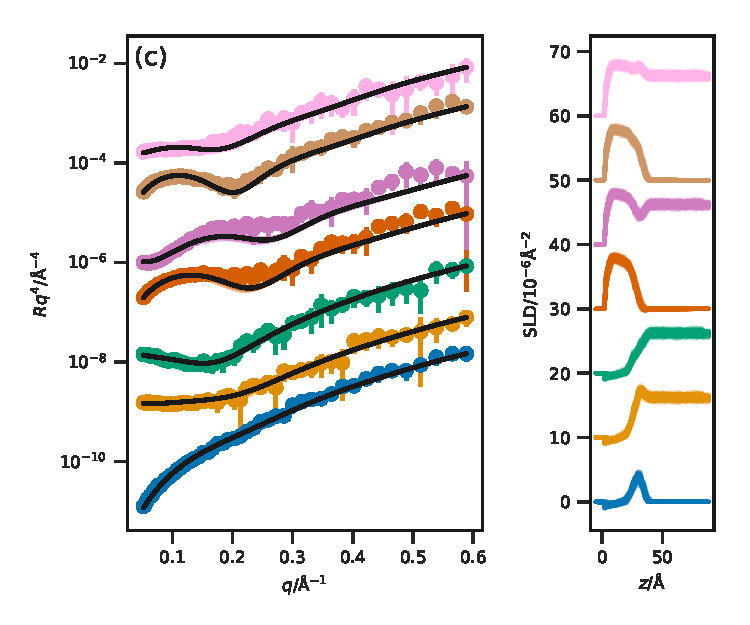
\includegraphics[width=0.49\textwidth]{reflectometry2/dspc_slipids_40_ref_sld}\\
    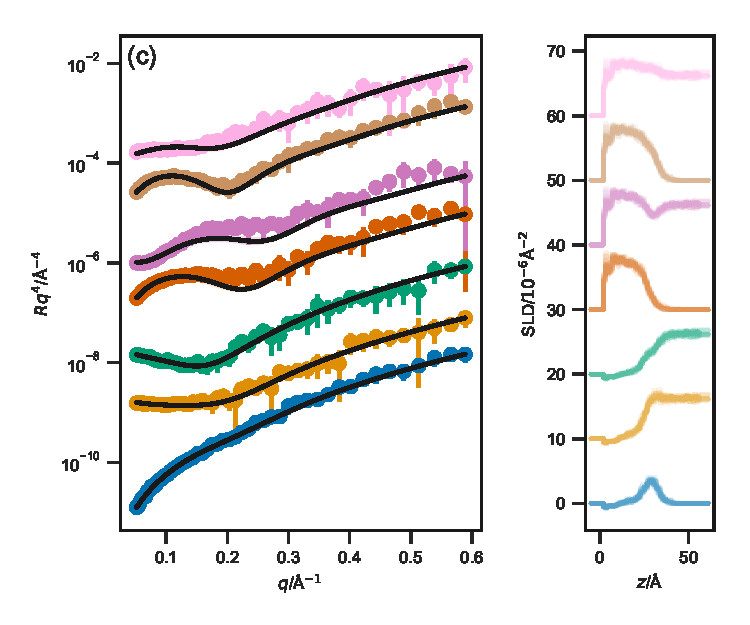
\includegraphics[width=0.49\textwidth]{reflectometry2/dspc_berger_40_ref_sld}
    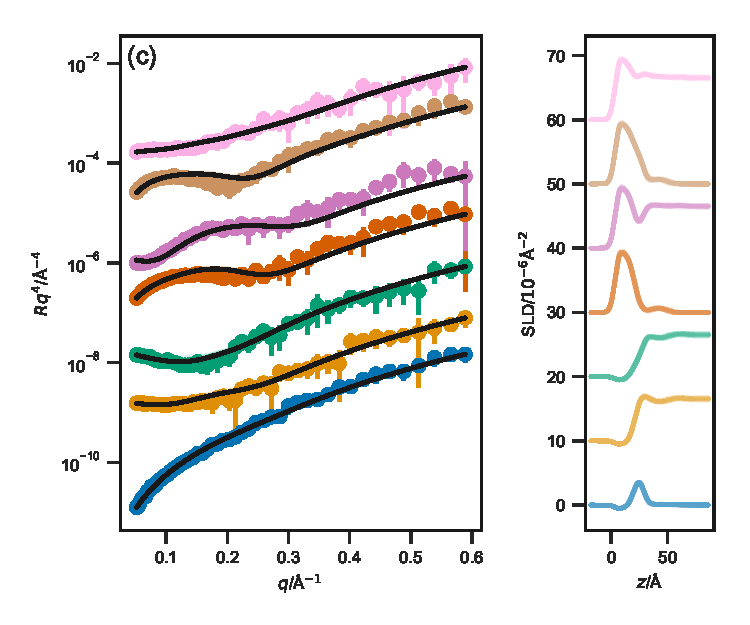
\includegraphics[width=0.49\textwidth]{reflectometry2/dspc_martini_40_ref_sld}
    \caption{The NR profiles (left) and SLD profiles (right) determined at an APM assocaited with a surface pressure of \SI{40}{\milli\newton\per\meter} for; (a) the chemically-consistent model, (b) the Slipid all-atom potential model simulations, (c) the Berger united-atom potential model simulations, and (d) the MARTINI coarse-grained potential model simulations. From top-to-bottom the contrasts are as follows; d$_{83}$-\ce{D2O}, d$_{83}$-ACMW, d$_{70}$-\ce{D2O}, d$_{70}$-ACMW, h-\ce{D2O}, d$_{13}$-\ce{D2O}, d$_{13}$-ACMW. The different contrast NR profiles have been offset in the \emph{y}-axis by an order of magnitude and the SLD profiles offset in the \emph{y}-axis by \SI{10e-6}{\per\angstrom\squared}, for clarity.}
    \label{fig:dspcccref40}
\end{figure}
%
%
\begin{figure}
    \centering
    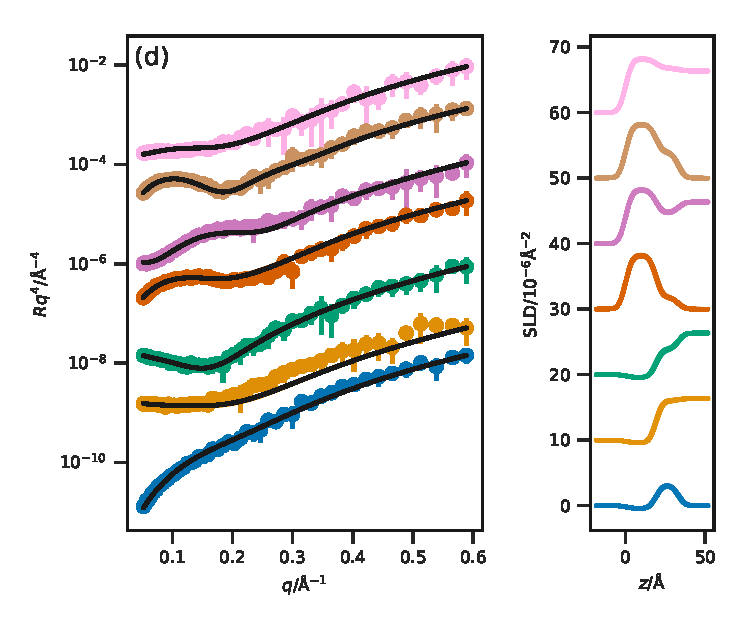
\includegraphics[width=0.49\textwidth]{reflectometry2/dspc_50_ref_sld}
    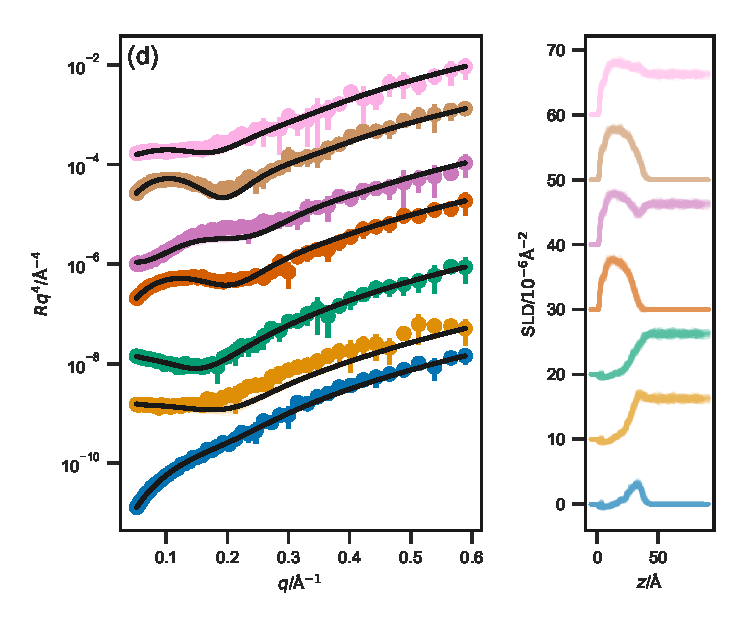
\includegraphics[width=0.49\textwidth]{reflectometry2/dspc_slipids_50_ref_sld}\\
    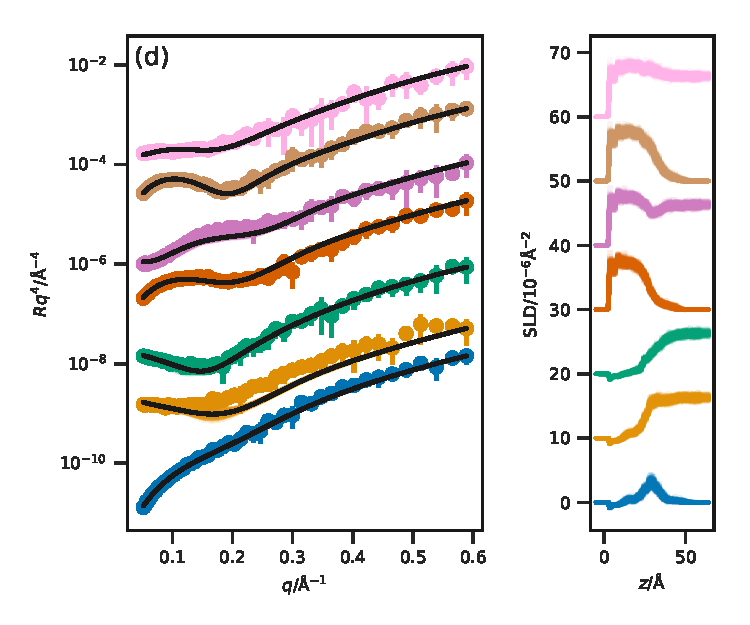
\includegraphics[width=0.49\textwidth]{reflectometry2/dspc_berger_50_ref_sld}
    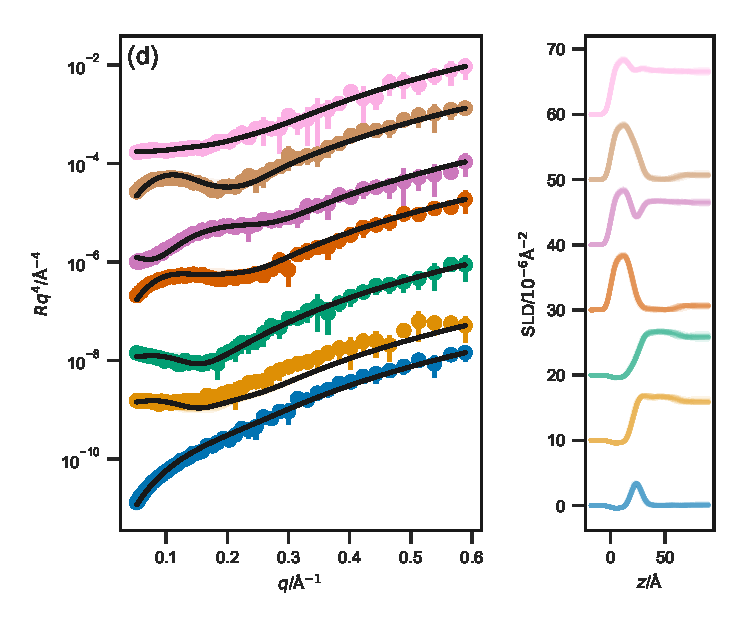
\includegraphics[width=0.49\textwidth]{reflectometry2/dspc_martini_50_ref_sld}
    \caption{The NR profiles (left) and SLD profiles (right) determined at an APM assocaited with a surface pressure of \SI{50}{\milli\newton\per\meter} for; (a) the chemically-consistent model, (b) the Slipid all-atom potential model simulations, (c) the Berger united-atom potential model simulations, and (d) the MARTINI coarse-grained potential model simulations. From top-to-bottom the contrasts are as follows; d$_{83}$-\ce{D2O}, d$_{83}$-ACMW, d$_{70}$-\ce{D2O}, d$_{70}$-ACMW, h-\ce{D2O}, d$_{13}$-\ce{D2O}, d$_{13}$-ACMW. The different contrast NR profiles have been offset in the \emph{y}-axis by an order of magnitude and the SLD profiles offset in the \emph{y}-axis by \SI{10e-6}{\per\angstrom\squared}, for clarity.}
    \label{fig:dspcccref50}
\end{figure}
%

Tables~\ref{tab:chi20}-\ref{tab:chi50} give the figure of merit for agreement between the model and the data from each of the analysis method at a APM associated with a surface pressure of \SIlist{20;40;50}{\milli\newton\per\meter}. 
The equivalent data at a APM associated with a surface pressure of \SI{30}{\milli\newton\per\meter} can be found in Table~\ref{tab:chi}. 
%
\begin{table}
    \centering
    \small
    \caption{The $\chi^2$ values for each of the reflectometry models at an APM associated with a surface pressure of \SI{20}{\milli\newton\per\meter}.}
    \label{tab:chi20}
    \begin{tabular}{l | l l l l}
        \toprule
        Contrast & Chemically-consistent & Slipids & Berger & MARTINI \\
        \midrule
        h-\ce{D2O} & \input{output/reflectometry2/dspc_20/dspc_20_hd2o_chi.txt} & \input{output/reflectometry2/dspc_20/dspc_slipids_20_hd2o_chi.txt} & \input{output/reflectometry2/dspc_20/dspc_berger_20_hd2o_chi.txt} & \input{output/reflectometry2/dspc_20/dspc_martini_20_hd2o_chi.txt} \\
        d$_{13}$-\ce{D2O} & \input{output/reflectometry2/dspc_20/dspc_20_d13d2o_chi.txt} & \input{output/reflectometry2/dspc_20/dspc_slipids_20_d13d2o_chi.txt} & \input{output/reflectometry2/dspc_20/dspc_berger_20_d13d2o_chi.txt} & \input{output/reflectometry2/dspc_20/dspc_martini_20_d13d2o_chi.txt} \\
        d$_{13}$-ACMW & \input{output/reflectometry2/dspc_20/dspc_20_d13acmw_chi.txt} & \input{output/reflectometry2/dspc_20/dspc_slipids_20_d13acmw_chi.txt} & \input{output/reflectometry2/dspc_20/dspc_berger_20_d13acmw_chi.txt} & \input{output/reflectometry2/dspc_20/dspc_martini_20_d13acmw_chi.txt} \\
        d$_{70}$-\ce{D2O} & \input{output/reflectometry2/dspc_20/dspc_20_d70d2o_chi.txt} & \input{output/reflectometry2/dspc_20/dspc_slipids_20_d70d2o_chi.txt} & \input{output/reflectometry2/dspc_20/dspc_berger_20_d70d2o_chi.txt} & \input{output/reflectometry2/dspc_20/dspc_martini_20_d70d2o_chi.txt} \\
        d$_{70}$-ACMW & \input{output/reflectometry2/dspc_20/dspc_20_d70acmw_chi.txt} & \input{output/reflectometry2/dspc_20/dspc_slipids_20_d70acmw_chi.txt} & \input{output/reflectometry2/dspc_20/dspc_berger_20_d70acmw_chi.txt} & \input{output/reflectometry2/dspc_20/dspc_martini_20_d70acmw_chi.txt} \\
        d$_{83}$-\ce{D2O} & \input{output/reflectometry2/dspc_20/dspc_20_d83d2o_chi.txt} & \input{output/reflectometry2/dspc_20/dspc_slipids_20_d83d2o_chi.txt} & \input{output/reflectometry2/dspc_20/dspc_berger_20_d83d2o_chi.txt} & \input{output/reflectometry2/dspc_20/dspc_martini_20_d83d2o_chi.txt} \\
        d$_{83}$-ACMW & \input{output/reflectometry2/dspc_20/dspc_20_d83acmw_chi.txt} & \input{output/reflectometry2/dspc_20/dspc_slipids_20_d83acmw_chi.txt} & \input{output/reflectometry2/dspc_20/dspc_berger_20_d83acmw_chi.txt} & \input{output/reflectometry2/dspc_20/dspc_martini_20_d83acmw_chi.txt} \\
        \midrule
        Average & \input{output/reflectometry2/dspc_20/dspc_20_all_chi.txt} & \input{output/reflectometry2/dspc_20/dspc_slipids_20_all_chi.txt} & \input{output/reflectometry2/dspc_20/dspc_berger_20_all_chi.txt} & \input{output/reflectometry2/dspc_20/dspc_martini_20_all_chi.txt} \\
        \bottomrule
    \end{tabular}
\end{table}
%
%
\begin{table}
    \centering
    \small
    \caption{The $\chi^2$ values for each of the reflectometry models at an APM associated with a surface pressure of \SI{40}{\milli\newton\per\meter}.}
    \label{tab:chi40}
    \begin{tabular}{l | l l l l}
        \toprule
        Contrast & Chemically-consistent & Slipids & Berger & MARTINI \\
        \midrule
        h-\ce{D2O} & \input{output/reflectometry2/dspc_40/dspc_40_hd2o_chi.txt} & \input{output/reflectometry2/dspc_40/dspc_slipids_40_hd2o_chi.txt} & \input{output/reflectometry2/dspc_40/dspc_berger_40_hd2o_chi.txt} & \input{output/reflectometry2/dspc_40/dspc_martini_40_hd2o_chi.txt} \\
        d$_{13}$-\ce{D2O} & \input{output/reflectometry2/dspc_40/dspc_40_d13d2o_chi.txt} & \input{output/reflectometry2/dspc_40/dspc_slipids_40_d13d2o_chi.txt} & \input{output/reflectometry2/dspc_40/dspc_berger_40_d13d2o_chi.txt} & \input{output/reflectometry2/dspc_40/dspc_martini_40_d13d2o_chi.txt} \\
        d$_{13}$-ACMW & \input{output/reflectometry2/dspc_40/dspc_40_d13acmw_chi.txt} & \input{output/reflectometry2/dspc_40/dspc_slipids_40_d13acmw_chi.txt} & \input{output/reflectometry2/dspc_40/dspc_berger_40_d13acmw_chi.txt} & \input{output/reflectometry2/dspc_40/dspc_martini_40_d13acmw_chi.txt} \\
        d$_{70}$-\ce{D2O} & \input{output/reflectometry2/dspc_40/dspc_40_d70d2o_chi.txt} & \input{output/reflectometry2/dspc_40/dspc_slipids_40_d70d2o_chi.txt} & \input{output/reflectometry2/dspc_40/dspc_berger_40_d70d2o_chi.txt} & \input{output/reflectometry2/dspc_40/dspc_martini_40_d70d2o_chi.txt} \\
        d$_{70}$-ACMW & \input{output/reflectometry2/dspc_40/dspc_40_d70acmw_chi.txt} & \input{output/reflectometry2/dspc_40/dspc_slipids_40_d70acmw_chi.txt} & \input{output/reflectometry2/dspc_40/dspc_berger_40_d70acmw_chi.txt} & \input{output/reflectometry2/dspc_40/dspc_martini_40_d70acmw_chi.txt} \\
        d$_{83}$-\ce{D2O} & \input{output/reflectometry2/dspc_40/dspc_40_d83d2o_chi.txt} & \input{output/reflectometry2/dspc_40/dspc_slipids_40_d83d2o_chi.txt} & \input{output/reflectometry2/dspc_40/dspc_berger_40_d83d2o_chi.txt} & \input{output/reflectometry2/dspc_40/dspc_martini_40_d83d2o_chi.txt} \\
        d$_{83}$-ACMW & \input{output/reflectometry2/dspc_40/dspc_40_d83acmw_chi.txt} & \input{output/reflectometry2/dspc_40/dspc_slipids_40_d83acmw_chi.txt} & \input{output/reflectometry2/dspc_40/dspc_berger_40_d83acmw_chi.txt} & \input{output/reflectometry2/dspc_40/dspc_martini_40_d83acmw_chi.txt} \\
        \midrule
        Average & \input{output/reflectometry2/dspc_40/dspc_40_all_chi.txt} & \input{output/reflectometry2/dspc_40/dspc_slipids_40_all_chi.txt} & \input{output/reflectometry2/dspc_40/dspc_berger_40_all_chi.txt} & \input{output/reflectometry2/dspc_40/dspc_martini_40_all_chi.txt} \\
        \bottomrule
    \end{tabular}
\end{table}
%
%
\begin{table}
    \centering
    \small
    \caption{The $\chi^2$ values for each of the reflectometry models at an APM associated with a surface pressure of \SI{50}{\milli\newton\per\meter}.}
    \label{tab:chi50}
    \begin{tabular}{l | l l l l}
        \toprule
        Contrast & Chemically-consistent & Slipids & Berger & MARTINI \\
        \midrule
        h-\ce{D2O} & \input{output/reflectometry2/dspc_50/dspc_50_hd2o_chi.txt} & \input{output/reflectometry2/dspc_50/dspc_slipids_50_hd2o_chi.txt} & \input{output/reflectometry2/dspc_50/dspc_berger_50_hd2o_chi.txt} & \input{output/reflectometry2/dspc_50/dspc_martini_50_hd2o_chi.txt} \\
        d$_{13}$-\ce{D2O} & \input{output/reflectometry2/dspc_50/dspc_50_d13d2o_chi.txt} & \input{output/reflectometry2/dspc_50/dspc_slipids_50_d13d2o_chi.txt} & \input{output/reflectometry2/dspc_50/dspc_berger_50_d13d2o_chi.txt} & \input{output/reflectometry2/dspc_50/dspc_martini_50_d13d2o_chi.txt} \\
        d$_{13}$-ACMW & \input{output/reflectometry2/dspc_50/dspc_50_d13acmw_chi.txt} & \input{output/reflectometry2/dspc_50/dspc_slipids_50_d13acmw_chi.txt} & \input{output/reflectometry2/dspc_50/dspc_berger_50_d13acmw_chi.txt} & \input{output/reflectometry2/dspc_50/dspc_martini_50_d13acmw_chi.txt} \\
        d$_{70}$-\ce{D2O} & \input{output/reflectometry2/dspc_50/dspc_50_d70d2o_chi.txt} & \input{output/reflectometry2/dspc_50/dspc_slipids_50_d70d2o_chi.txt} & \input{output/reflectometry2/dspc_50/dspc_berger_50_d70d2o_chi.txt} & \input{output/reflectometry2/dspc_50/dspc_martini_50_d70d2o_chi.txt} \\
        d$_{70}$-ACMW & \input{output/reflectometry2/dspc_50/dspc_50_d70acmw_chi.txt} & \input{output/reflectometry2/dspc_50/dspc_slipids_50_d70acmw_chi.txt} & \input{output/reflectometry2/dspc_50/dspc_berger_50_d70acmw_chi.txt} & \input{output/reflectometry2/dspc_50/dspc_martini_50_d70acmw_chi.txt} \\
        d$_{83}$-\ce{D2O} & \input{output/reflectometry2/dspc_50/dspc_50_d83d2o_chi.txt} & \input{output/reflectometry2/dspc_50/dspc_slipids_50_d83d2o_chi.txt} & \input{output/reflectometry2/dspc_50/dspc_berger_50_d83d2o_chi.txt} & \input{output/reflectometry2/dspc_50/dspc_martini_50_d83d2o_chi.txt} \\
        d$_{83}$-ACMW & \input{output/reflectometry2/dspc_50/dspc_50_d83acmw_chi.txt} & \input{output/reflectometry2/dspc_50/dspc_slipids_50_d83acmw_chi.txt} & \input{output/reflectometry2/dspc_50/dspc_berger_50_d83acmw_chi.txt} & \input{output/reflectometry2/dspc_50/dspc_martini_50_d83acmw_chi.txt} \\
        \midrule
        Average & \input{output/reflectometry2/dspc_50/dspc_50_all_chi.txt} & \input{output/reflectometry2/dspc_50/dspc_slipids_50_all_chi.txt} & \input{output/reflectometry2/dspc_50/dspc_berger_50_all_chi.txt} & \input{output/reflectometry2/dspc_50/dspc_martini_50_all_chi.txt} \\
        \bottomrule
    \end{tabular}
\end{table}
%

The solvent penetration at APMs associated with surface pressures of \SIlist{20;40;50}{\milli\newton\per\meter} is shown in Figures~\ref{fig:waters20}-\ref{fig:waters50} using the intrinsic density profile. 
The equivalent figure for an APM associated with a surface pressure of \SI{30}{\milli\newton\per\meter} can be found in Figure~\ref{fig:waters30}.
%
\begin{figure}
    \centering
    \includegraphics[width=\textwidth]{reflectometry2/water_20}
    \caption{The simulation time-averaged intrinsic density profile of the water molecules (blue dots), and phospholipid components (head groups: green dots, tail groups: red dots) at an APM associated with a surface pressure of \SI{20}{\milli\newton\per\meter}, where the phosphorus atoms of the phospholipid heads create the intrinsic surface at $z=0$\si{\angstrom}, and the equivalent number density from the chemically-consistent model (orange line).}
    \label{fig:waters20}
\end{figure}
%
%
\begin{figure}
    \centering
    \includegraphics[width=\textwidth]{reflectometry2/water_40}
    \caption{The simulation time-averaged intrinsic density profile of the water molecules (blue dots), and phospholipid components (head groups: green dots, tail groups: red dots) at an APM associated with a surface pressure of \SI{40}{\milli\newton\per\meter}, where the phosphorus atoms of the phospholipid heads create the intrinsic surface at $z=0$\si{\angstrom}, and the equivalent number density from the chemically-consistent model (orange line).}
    \label{fig:waters40}
\end{figure}
%
%
\begin{figure}
    \centering
    \includegraphics[width=\textwidth]{reflectometry2/water_50}
    \caption{The simulation time-averaged intrinsic density profile of the water molecules (blue dots), and phospholipid components (head groups: green dots, tail groups: red dots) at an APM associated with a surface pressure of \SI{50}{\milli\newton\per\meter}, where the phosphorus atoms of the phospholipid heads create the intrinsic surface at $z=0$\si{\angstrom}, and the equivalent number density from the chemically-consistent model (orange line).}
    \label{fig:waters50}
\end{figure}
%

The quantification of the interfacial roughness determined from the Slipids simulations at APMs associated with surface pressures of \SIlist{20;40;50}{\milli\newton\per\meter} are given in Tables~\\ref{tab:spread1}-\ref{tab:spread4}. 
The equivalent data for an APM associated with a surface pressure of \SI{30}{\milli\newton\per\meter} can be found in Table~\ref{tab:spread2}.
%
\begin{table}
\centering
\small
  \caption{\ The mean, \SI{95}{\percent} quantile, and their spread for the \emph{z}-dimension position of atoms representative of difference parts of the phospholipid, at an APM associated with a surface pressure of \SI{20}{\milli\newton\per\meter}.}
  \label{tab:spread1}
  \begin{tabular}{llll}
    \toprule
    Position & Mean/\si{\angstrom} & \SI{95}{\percent} quantile/\si{\angstrom} & Spread/\si{\angstrom} \\
    \midrule
    Start-Head & \input{output/reflectometry2/dspc_20/slipids_mean_N_20.txt} & \input{output/reflectometry2/dspc_20/slipids_uq_N_20.txt} & \input{output/reflectometry2/dspc_20/slipids_position_N_20.txt} \\
    Mid-Head & \input{output/reflectometry2/dspc_20/slipids_mean_P_20.txt} & \input{output/reflectometry2/dspc_20/slipids_uq_P_20.txt} & \input{output/reflectometry2/dspc_20/slipids_position_P_20.txt} \\
    End-Head & \input{output/reflectometry2/dspc_20/slipids_mean_C2_20.txt} & \input{output/reflectometry2/dspc_20/slipids_uq_C2_20.txt} & \input{output/reflectometry2/dspc_20/slipids_position_C2_20.txt} \\
    \midrule
    Start-Tail 1 & \input{output/reflectometry2/dspc_20/slipids_mean_C21_20.txt} & \input{output/reflectometry2/dspc_20/slipids_uq_C21_20.txt} & \input{output/reflectometry2/dspc_20/slipids_position_C21_20.txt} \\
    Start-Tail 2 & \input{output/reflectometry2/dspc_20/slipids_mean_C31_20.txt} & \input{output/reflectometry2/dspc_20/slipids_uq_C31_20.txt} & \input{output/reflectometry2/dspc_20/slipids_position_C31_20.txt} \\
    Mid-Tail 1 & \input{output/reflectometry2/dspc_20/slipids_mean_C29_20.txt} & \input{output/reflectometry2/dspc_20/slipids_uq_C29_20.txt} & \input{output/reflectometry2/dspc_20/slipids_position_C29_20.txt} \\
    Mid-Tail 2 & \input{output/reflectometry2/dspc_20/slipids_mean_C39_20.txt} & \input{output/reflectometry2/dspc_20/slipids_uq_C39_20.txt} & \input{output/reflectometry2/dspc_20/slipids_position_C39_20.txt} \\
    End-Tail 1 & \input{output/reflectometry2/dspc_20/slipids_mean_8C21_20.txt} & \input{output/reflectometry2/dspc_20/slipids_uq_8C21_20.txt} & \input{output/reflectometry2/dspc_20/slipids_position_8C21_20.txt} \\
    End-Tail 2 & \input{output/reflectometry2/dspc_20/slipids_mean_8C31_20.txt} & \input{output/reflectometry2/dspc_20/slipids_uq_8C31_20.txt} & \input{output/reflectometry2/dspc_20/slipids_position_8C31_20.txt} \\
    \bottomrule
  \end{tabular}
\end{table}
%
%
\begin{table}
\centering
\small
  \caption{\ The mean, \SI{95}{\percent} quantile, and their spread for the \emph{z}-dimension position of atoms representative of difference parts of the phospholipid, at an APM associated with a surface pressure of \SI{40}{\milli\newton\per\meter}.}
  \label{tab:spread3}
  \begin{tabular}{llll}
    \toprule
    Position & Mean/\si{\angstrom} & \SI{95}{\percent} quantile/\si{\angstrom} & Spread/\si{\angstrom} \\
    \midrule
    Start-Head & \input{output/reflectometry2/dspc_40/slipids_mean_N_40.txt} & \input{output/reflectometry2/dspc_40/slipids_uq_N_40.txt} & \input{output/reflectometry2/dspc_40/slipids_position_N_40.txt} \\
    Mid-Head & \input{output/reflectometry2/dspc_40/slipids_mean_P_40.txt} & \input{output/reflectometry2/dspc_40/slipids_uq_P_40.txt} & \input{output/reflectometry2/dspc_40/slipids_position_P_40.txt} \\
    End-Head & \input{output/reflectometry2/dspc_40/slipids_mean_C2_40.txt} & \input{output/reflectometry2/dspc_40/slipids_uq_C2_40.txt} & \input{output/reflectometry2/dspc_40/slipids_position_C2_40.txt} \\
    \midrule
    Start-Tail 1 & \input{output/reflectometry2/dspc_40/slipids_mean_C21_40.txt} & \input{output/reflectometry2/dspc_40/slipids_uq_C21_40.txt} & \input{output/reflectometry2/dspc_40/slipids_position_C21_40.txt} \\
    Start-Tail 2 & \input{output/reflectometry2/dspc_40/slipids_mean_C31_40.txt} & \input{output/reflectometry2/dspc_40/slipids_uq_C31_40.txt} & \input{output/reflectometry2/dspc_40/slipids_position_C31_40.txt} \\
    Mid-Tail 1 & \input{output/reflectometry2/dspc_40/slipids_mean_C29_40.txt} & \input{output/reflectometry2/dspc_40/slipids_uq_C29_40.txt} & \input{output/reflectometry2/dspc_40/slipids_position_C29_40.txt} \\
    Mid-Tail 2 & \input{output/reflectometry2/dspc_40/slipids_mean_C39_40.txt} & \input{output/reflectometry2/dspc_40/slipids_uq_C39_40.txt} & \input{output/reflectometry2/dspc_40/slipids_position_C39_40.txt} \\
    End-Tail 1 & \input{output/reflectometry2/dspc_40/slipids_mean_8C21_40.txt} & \input{output/reflectometry2/dspc_40/slipids_uq_8C21_40.txt} & \input{output/reflectometry2/dspc_40/slipids_position_8C21_40.txt} \\
    End-Tail 2 & \input{output/reflectometry2/dspc_40/slipids_mean_8C31_40.txt} & \input{output/reflectometry2/dspc_40/slipids_uq_8C31_40.txt} & \input{output/reflectometry2/dspc_40/slipids_position_8C31_40.txt} \\
    \bottomrule
  \end{tabular}
\end{table}
%
%
\begin{table}
\centering
\small
  \caption{\ The mean, \SI{95}{\percent} quantile, and their spread for the \emph{z}-dimension position of atoms representative of difference parts of the phospholipid, at an APM associated with a surface pressure of \SI{50}{\milli\newton\per\meter}.}
  \label{tab:spread4}
  \begin{tabular}{llll}
    \toprule
    Position & Mean/\si{\angstrom} & \SI{95}{\percent} quantile/\si{\angstrom} & Spread/\si{\angstrom} \\
    \midrule
    Start-Head & \input{output/reflectometry2/dspc_50/slipids_mean_N_50.txt} & \input{output/reflectometry2/dspc_50/slipids_uq_N_50.txt} & \input{output/reflectometry2/dspc_50/slipids_position_N_50.txt} \\
    Mid-Head & \input{output/reflectometry2/dspc_50/slipids_mean_P_50.txt} & \input{output/reflectometry2/dspc_50/slipids_uq_P_50.txt} & \input{output/reflectometry2/dspc_50/slipids_position_P_50.txt} \\
    End-Head & \input{output/reflectometry2/dspc_50/slipids_mean_C2_50.txt} & \input{output/reflectometry2/dspc_50/slipids_uq_C2_50.txt} & \input{output/reflectometry2/dspc_50/slipids_position_C2_50.txt} \\
    \midrule
    Start-Tail 1 & \input{output/reflectometry2/dspc_50/slipids_mean_C21_50.txt} & \input{output/reflectometry2/dspc_50/slipids_uq_C21_50.txt} & \input{output/reflectometry2/dspc_50/slipids_position_C21_50.txt} \\
    Start-Tail 2 & \input{output/reflectometry2/dspc_50/slipids_mean_C31_50.txt} & \input{output/reflectometry2/dspc_50/slipids_uq_C31_50.txt} & \input{output/reflectometry2/dspc_50/slipids_position_C31_50.txt} \\
    Mid-Tail 1 & \input{output/reflectometry2/dspc_50/slipids_mean_C29_50.txt} & \input{output/reflectometry2/dspc_50/slipids_uq_C29_50.txt} & \input{output/reflectometry2/dspc_50/slipids_position_C29_50.txt} \\
    Mid-Tail 2 & \input{output/reflectometry2/dspc_50/slipids_mean_C39_50.txt} & \input{output/reflectometry2/dspc_50/slipids_uq_C39_50.txt} & \input{output/reflectometry2/dspc_50/slipids_position_C39_50.txt} \\
    End-Tail 1 & \input{output/reflectometry2/dspc_50/slipids_mean_8C21_50.txt} & \input{output/reflectometry2/dspc_50/slipids_uq_8C21_50.txt} & \input{output/reflectometry2/dspc_50/slipids_position_8C21_50.txt} \\
    End-Tail 2 & \input{output/reflectometry2/dspc_50/slipids_mean_8C31_50.txt} & \input{output/reflectometry2/dspc_50/slipids_uq_8C31_50.txt} & \input{output/reflectometry2/dspc_50/slipids_position_8C31_50.txt} \\
    \bottomrule
  \end{tabular}
\end{table}
%
